
\chapter{Cryptographie sur les courbes elliptiques}
Une courbe elliptique est une courbe plane régit par une équation de forme particulière, dont les points possèdent la propriété remarquable de pouvoir être additionnés entre eux. On peut donc, étant donné un point $P$ et un entier $n$, définir le point $Q = nP$ comme $Q = P + P + \ldots + P$ (où $P$ apparaît $n$ fois). En cryptographie, on utilise des points à coordonnées discrètes de grandes tailles (typiquement un corps premier ou aussi une extension d'un corps binaire, de 200 bits). $P$ étant donné, $Q$ peut être rapidement calculé par ordinateur même lorsque $n$ est lui aussi de grande taille. L'inverse est faux : de façon surprenante on ne connaît aucune méthode efficace de retrouver $n$ à partir de $P$ et $Q$. Ce problème difficile, appelé \emph{problème du logarithme discret sur courbe elliptique} \footnote{On trouve aussi parfois le terme logarithme elliptique.}, permet de concevoir des algorithmes à clé publique en choisissant $n$ comme clé secrète et $Q$ comme clé publique.

Introduite dés 1985, l'ECC \footnote{Elliptic Curve Cryptography : Cryptographie sur Courbes Elliptiques} se déploie progressivement. On la retrouve aussi bien dans le monde Internet/Web (TLS, SSH, Bitcoin) que dans la télévision à péage (Viaccess), la téléphonie (SIM) ou l'identification (passeports).

\todo{Expliqué rapidement l'utilisation des courbes elliptiques en crypto. Expliquer qu'il existe différentes familles de courbes qui possèdent chacunes leurs spécificités : formule unifiée, différents système de coordonnées, choix de l'algorithme de multiplication scalaire régulier ou non, utilisation d'endomorphisme, choix de représentation des éléments \ldots}

\section{Vue générale}
L'utilisation des courbes elliptiques en cryptographie a été proposée en 1985 indépendamment par Victor Miller et Neal Koblitz. L'ensemble des points d'une courbe elliptique peut être munie d'une structure de groupe (d'une addition). L'addition de points d'une courbe elliptique à coordonnées réelles s'interprètent facilement de manière géométrique. L'idée consiste d'utiliser le groupe des points d'une courbe au problème de logarithme discret. La principale raison de son attrait est qu'on ne connaît aucun algorithme sous-exponentiel résolvant le problème du logarithme discret sur des courbes elliptiques bien choisies. Ce qui conduit à des tailles de paramètres significativement plus petit que les cryptosystèmes tel que RSA ou DSA pour un même niveau de sécurité. Ainsi plus le niveau de sécurité est grand et plus ce fossé est important. Des tailles de clé plus faibles permettent des calculs plus rapides, une réduction de l'espace de stockage, de bande passante et de puissance de traitement \footnote{Bandwith, processing power.}.

L'utilisation des courbes elliptiques nécessite d'effectuer un certain nombre de choix : choix du cryptosystème, du modèle de la courbe et de ses coefficients, du corps fini, de l'algorithme de multiplication scalaire, des algorithmes pour les opérations dans le corps de base \ldots Chacune de ces applications peuvent avoir un impact significatif sur la performance globale de notre application.

Avant de pouvoir décrire une méthode, un procédé de génération de courbes elliptiques, il faut au préalable recenser l'ensemble des attaques connues. Chacune de ces attaques met en lumière une faille potentielle dans l'utilisation des ECC. Elles signalent que tel ou tel choix de courbes, de paramètres doivent être éviter, que ces derniers doivent vérifier une certaines propriétés. On obtient une condition nécessaire pour atteindre un niveau de sécurité. La condition suffisante se fait via la notion de réduction.

La cryptographie sur courbes elliptiques se décompose en plusieurs couches. Choix du protocole, algorithme de multiplication scalaire, formules d'addition et de doublement et enfin opérations dans le corps de base. 

\begin{figure}[h]
    \centering
    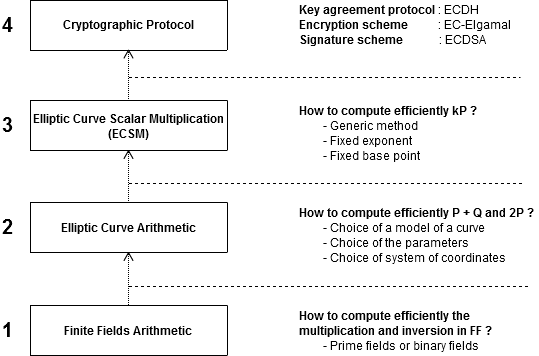
\includegraphics[scale=0.7]{images/ECC_level.png}
    \caption{Hiérarchie, couches dans l'utilisation des courbes elliptiques en cryptographie}
    \label{fig:my_label}
\end{figure}
\FloatBarrier

\section{Intérêt des courbes elliptiques en cryptographie}
Nous résumons ici les attraits (et points faibles) de la cryptographie sur courbe elliptique par rapport à la cryptographie asymétrique classique.
\begin{itemize}[label=$\bullet$]
    \item Excepté pour quelques familles courbes, il n'y pas de meilleurs attaques connues que les attaques génériques pour résoudre le problème du logarithme discret.
    \item Le corps de base est plus petit que celui de RSA ou du logarithme discret sur un corps finis pour un même niveau de sécurité : $224$ bits au lieu de $2048$ pour $128$ bits de sécurité. Actuellement le gain est de l'ordre d'un facteur $10$.
    \begin{itemize}[label=--]
        \item Arithmétique du corps de base plus facile à implémenter et plus efficace.
        \item Clés plus petites qu'avec RSA (sauf pour la clé publique), actuellement différence de l'ordre d'un facteur $10$.
        \item Génération de clé facile (contrairement à RSA).
        \item ECC plus rapide que le DL sur corps finis.
        \item ECC plus rapide que RSA pour les opérations privées mais pas pour les opérations publiques si on choisit $e = 3$. La vérification des signatures est donc un peu plus efficace.
    \end{itemize}
    \item Ce fossé entre ECC et les autres systèmes s'accroît (attaques exponentielles contre sous-exponentielle). Plus le temps passe, plus la puissance des ordinateurs est grande. Augmenter le niveau de sécurité requiert d'augmenter davantage la taille de clés de RSA que de ECC.
    \item Création de protocoles originaux en utilisant les couplages : échange de clé tri-partite, chiffrement basé sur l'identité, signatures courtes.
\end{itemize}

ECC versus RSA : \cite{koblitz2011elliptic}. Au départ l'arrivée des courbes elliptiques en cryptographie a suscité parmi les cryptographes la curiosité et l'approbation. Bien que la plupart des chercheurs n'avait jamais étudié les courbes elliptiques et n'en avait qu'une compréhension limitée, ils avaient tendance à réagir positivement. 
Puis création de la compagnie Certicom : ECC devient alors une menace commerciale à le RSA. 


{\renewcommand{\arraystretch}{1.3}
\begin{table}[h]
\centering
    \begin{tabular}{|c||c|c|c|c|c|}
        \hline
        Niveau de Sécurité en bits & $80$ & $112$ & $128$ & $192$ & $256$\\
        \hline
        Module RSA en bits & 1024 & 2048 & 3072 & 8192 & 15360 \\
        \hline
        ECC : Taille du corps de base en bits & $160$ & $224$ & $256$ & $384$ & $521$ \\
        \hline
    \end{tabular}
\caption{Comparatifs des tailles des clés pour différents niveau de sécurité entre RSA et ECC}
\label{tab:keylength}
\end{table}}
Le site \href{http://www.keylength.com}{KeyLength} liste les recommandations d'agences gouvernementales concernant la taille minimale des clés a adopté. La plupart préconise $112$ bits de sécurité environ.

\begin{comment}
\begin{figure}[scale=0.4]
\centering
    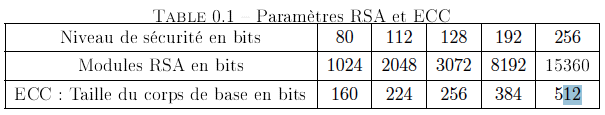
\includegraphics[scale=0.5]{images/paramRSAECC.png}
    \caption{Comparatifs des tailles des clés pour différents niveau de sécurité entre RSA et ECC}
    \label{fig:keylength}
\end{figure}
\end{comment}

\section{Standards et brevets}
Au cours des années 2000, différentes courbes ont été standardisées. Certaines sont d'ailleurs données sans aucunes justifications. 
\begin{description}
    \item[NIST\footnote{NIST : National Institute of Standards and Technologie.}] \hfill \\ Spécification en 1999 de $15$ courbes : $5$ sur corps premiers, $5$ sur corps binaire et $5$ courbes de Koblitz. Forme de Weierstrass, nombre de Mersenne Généralisé, $a=-3$ et $b$ pseudo-random, co-facteur minimal ($2$ pour corps binaires et $2$ ou $4$ pour Koblitz).
    \item[SECG\footnote{SECG : Standards for Efficient Cryptography Group.}] \hfill \\
    Provient de la société canadienne Certicom, rachetée par BlackBerry. Date de 2009. Ce standard reprend certaines courbes du NIST (par exemple P-$256$ et secp256r1 correspondent à la même courbe). De plus il possède la particularité de proposer des courbes GLV avec $a = 0$ ou $b = 0$. Le protocole Bitcoin utilise une de ces courbes particulière, la secp256k1, mais sans tirer partie de l'endomorphisme facilement calculable associé.
    \item[Brainpool\footnote{Consortium Européen dirigé par la BSI qui l'analogue de l'ANSSI germanique.}] \hfill \\
    Date de 2005 (puis révisé en 2010). Procédé de génération de courbes plus rigides, du moins en apparence (les décimales de $\pi$ forment la graine pour le choix des nombres premiers et $\exp(1)$, la constante d'Euler, pour les coefficients de la courbe), forme de Weierstrass, $a$ et $p$ pseudo-aléatoire, non twist-secure.
    \item[Organismes Gouvernementaux] \hfill \\
    Données sans aucunes justifications. La Chine en 2010 a proposé OSCCA SM2 et la France par le biais de l'ANSSI en 2011, ANSSIFRP256v1 ou FRP256v1, paru aux JO \href{http://www.legifrance.gouv.fr/affichTexte.do;jsessionid=?cidTexte=JORFTEXT000024668816&dateTexte=&oldAction=rechJO&categorieLien=id}{ici}. Nombre premier pseudo-random et $a=-3$.
    \item[Académiques et Industriels] \hfill
        \begin{itemize}[label=--]
            \item Curve25519\footnote{Conventions : Curve$|d|$ pour les courbes d'Edwards avec le coefficient $d$, la taille du corps de base n'est donc pas spécifiée. Et on a Curve$m\delta$ pour les courbes de Montgomery sur $\GF{2^m - \delta}$. La convention utilisée ne permet pas toujours d'identifier clairement le modèle de courbe choisi.}, Curve41417 proposées par Bernstein et Lange. La première est une courbe de Montgomery définie sur $\GF{2^{255}-19}$ et est birationnellement équivalente à Ed25519.
            \item NUMS\footnote{NUMS : Nothing Up My Sleeve} Curves, proposées par l'équipe de Microsoft et Bos de NXP. \href{http://research.microsoft.com/pubs/219966/curvegen.pdf}{Lien.}
            \item Goldilocks448 ou Ed448-Goldilocks proposée par Hamburg. Appelé ainsi en référence au nombre d'or et à la forme du nombre premier. $p = 2^{448} - 2^{224} -1$.
            \item M-221, M-383, M-511, E-222, E-382, E-521. M pour Montgomery et E pour Edwards. Proposition de six nouvelles courbes à des niveaux sécurités similaires de ceux du NIST, complète les Curves. \href{https://eprint.iacr.org/2013/647.pdf}{Lien.} Ce papier résume les caractéristiques de la Curve25519. Il existe la Ridinghood curve seul change le nombre premier. $p = 2^{480} -2^{240} -1$.
            \item Ted127-glv4, Four$\mathbb{Q}$.
        \end{itemize}
\end{description}

Présentation intéressante, \href{http://www.imsc.res.in/~ecc14/slides/costello.pdf}{lien.} IRTF CFRG préconise l'adoption des courbes Curves25519 et Goldilocks448 pour l'inclusion dans les futures versions de TLS.

\vspace{0.5cm}

L'existence de brevets dans l'univers de la cryptographie sur courbe elliptique est un des facteurs limitant une acceptation plus générale, notamment pour les courbes binaires. Déposés notamment par le sociétés Certicom et Cryptography Research, ils protègent plus souvent des techniques d'implémentation que des courbes et des algorithmes proprement dits. Les brevets ne sont pas un frein très grand au déploiement et à l'adoption des courbes elliptiques en cryptographie. Aux quelques brevets existant, des solutions alternatives existent. 

Rappelons que Certicom \footnote{Racheté par Blackberry en 2009} est une société canadienne fondée par Scott Vanstonne, connu notamment pour l'algorithme DSA\footnote{Digital Signature Algorithm}. Cryptography Research est la société fondée par Paul Kocher. 

\noindent Quelques techniques sujettes aux brevets : 
\begin{itemize}[label=--]
    \item Nombres premiers sous une forme spéciale : Mersenne, pseudo-Mersenne ou Crandall, Mersenne Généralisé.
    \item Bases normales.
    \item Techniques de compression.
    \item Protocole d'échange de clé MQV.
    \item Techniques GLV.
\end{itemize}

Noter que la NSA en 2003 a racheté les droits de certains brevets sur ECC (notamment ceux sur MQV) dans un deal de $25$ millions de dollars et distribuent des licences à des compagnies américaines.

Remarques de Bernstein \footnote{\href{https://cr.yp.to/newelliptic/nistecc-20160106.pdf}{Failures in NIST ECC standards.}} : As far as we know, the most important ECC patents have all expired, and the entire core of ECC is now patent-free. Some fringes of ECC are still patented. The most interesting remaining patents are the GLV patents; these patents cover the use of endomorphisms to speed up ECC on special curves (GLV curves, GLS curves, \Q-curves, and so on).



\section{Dates notables}
\begin{itemize}
\item 85 : Introduction des courbes elliptiques en cryptographie indépendamment par Koblitz et Miller.
\item 87 : Courbes de Montgomery.
\item 89 : Introduction des courbes hyperelliptiques en cryptographie par Koblitz.
\item années 90 : apparition des couplages.
\item 93 : Attaque de Menezes-Okamoto-Vanstone (MOV) puis amélioration par Frey-Rück sur les courbes munient d'un petit degré de plongement.
\item 99 : Attaque de Smart-Semaev-Satoh-Araki sur les courbes anomales.
\item 99 : Spécifications des courbes du NIST.
\item 00 : \'Echange de clé tripartite à un tour d'A. joux.
\item 01 : Première réalisation effective d'un cryptosystème basé sur l'identité (IBE)\footnote{Identity Based Encryption : problème posé par Shamir en 84.} proposé par Boneh et Franklin à Crypto. Le cryptologue britannique Cocks\footnote{Qui a notamment découvert une variante de RSA quelques années plus tôt au sein du GCHQ.}, a proposé la même année un système IBE basé sur la résiduosité quadratique modulo deux nombres premiers.
\item 01 : Gallant, Lambert, Vanstone ont proposé une méthode appelé GLV à Crypto afin d'accélérer la multiplication scalaire à l'aide d'endomorphisme.
\item 06 : Proposition de la courbe Curve25519 (Montgomery) par Bernstein. 
\item 07 : Courbe d'Edwards, et les tordues d'Edwards l'année suivante.
\item 09 : standard de Certicom, nommé SECG v2.
\item 09 : Galbraith, Lin et Scott étendent la méthode GLV en construisant des endomorphismes efficient sur les twists de $E(\GF{p^2}$. La méthode GLS peut être appliquée aux courbes GLV on est ainsi muni de deux endomorphismes efficient permettant une décomposition en dimension 4.
\item 05 et 10 : courbes du Brainpool. Consortium européen dirigé par la BSI (analogue germanique de l'ANSSI).
\item 13 : \Q{}-curves proposées par Smith.
\end{itemize}